\documentclass[10pt,a4paper,landscape]{article}
\usepackage{multicol}
\usepackage{calc}
\usepackage{ifthen}
\usepackage[landscape]{geometry}
\usepackage{amsmath,amsthm,amsfonts,amssymb,mathtools}
\usepackage{color,graphicx}
\usepackage{hyperref}
\usepackage{listings}
\usepackage{underscore}
\usepackage{todonotes}

% Cheatsheet style
% Cheatsheet style

% This sets page margins to .5 inch if using letter paper, and to 1cm
% if using A4 paper. (This probably isn't strictly necessary.)
% If using another size paper, use default 1cm margins.
\ifthenelse{\lengthtest{\paperwidth = 11in}}
  % Then
  { \geometry{top=.5in,left=.5in,right=.5in,bottom=.5in} }
  % Else
  { \ifthenelse{\lengthtest{\paperwidth = 297mm}}
    {\geometry{top=0.1cm,left=0.1cm,right=0.1cm,bottom=0.2cm} }
    {\geometry{top=0.1cm,left=0.1cm,right=0.1cm,bottom=0.2cm} }
  }

% Turn off header and footer
\pagestyle{empty}

% Redefine section commands to use less space
\makeatletter
\renewcommand{\section}{\@startsection{section}{1}{0mm}%
                                {-1ex plus -.5ex minus -.2ex}%
                                {0.5ex plus .2ex}%x
                                {\color{darkred}\normalfont\large\bfseries}}
\renewcommand{\subsection}{\@startsection{subsection}{2}{0mm}%
                                {-1explus -.5ex minus -.2ex}%
                                {0.5ex plus .2ex}%
                                {\color{darkdarkred}\normalfont\normalsize\bfseries}}
\renewcommand{\subsubsection}{\@startsection{subsubsection}{3}{0mm}%
                                {-1ex plus -.5ex minus -.2ex}%
                                {1ex plus .2ex}%
                                {\normalfont\small\bfseries}}
\makeatother

% Define BibTeX command
\def\BibTeX{{\rm B\kern-.05em{\sc i\kern-.025em b}\kern-.08em
    T\kern-.1667em\lower.7ex\hbox{E}\kern-.125emX}}

% Don't print section numbers
\setcounter{secnumdepth}{0}

\setlength{\parindent}{0pt}
\setlength{\parskip}{0pt plus 0.5ex}

% Setting colors
\definecolor{lightgray}{rgb}{0.7,0.7,0.7}
\definecolor{lightergray}{rgb}{0.9,0.9,0.9}
\definecolor{darkblue}{rgb}{0.4,0.4,1}
\definecolor{darkred}{rgb}{0.9,0.2,0.2}
\definecolor{darkdarkred}{rgb}{0.6,0.0,0.0}
\definecolor{lightred}{rgb}{1,0.6,0.6}
\definecolor{lightgreen}{rgb}{0.6,1,0.6}
\definecolor{lightblue}{rgb}{0.6,0.8,1}
\definecolor{darkgreen}{rgb}{0.4,1,0.4}

% Set code listing style
\lstset {
    backgroundcolor=\color{lightgray},
    basicstyle=\ttfamily\scriptsize,
    breaklines=true,
}

\lstdefinestyle{bb}{
    backgroundcolor=\color{lightergray},
    frame=L,
    xleftmargin=\parindent,
}

% Remove `itemize` indentation
\usepackage{enumitem}
\setlist[itemize]{leftmargin=*}

% Set hyperlink style
\hypersetup{hidelinks}

% Enable figures
\newenvironment{colfig}
  {\par\medskip\noindent\minipage{\linewidth}}
  {\endminipage\par\medskip}

% Enable arg min/max math operators
\DeclareMathOperator*{\argmin}{arg\,min}
\DeclareMathOperator*{\argmax}{arg\,max}


% Shorthands
\renewcommand{\bf}[1]{\ensuremath{\mathbf{#1}}}
\newcommand{\E}{\mathrm{E}}
\newcommand{\Var}{\mathrm{Var}}
\newcommand{\Cov}{\mathrm{Cov}}
\newcommand{\balpha}{\boldsymbol\alpha}
\newcommand{\bbeta}{\boldsymbol\beta}
\newcommand{\bdelta}{\boldsymbol\delta}
\newcommand{\btheta}{\boldsymbol\theta}
\newcommand{\bPhi}{\boldsymbol\Phi}
 
\pdfinfo{
  /Title (Machine Learning Cheat Sheet)
  /Creator (TeX)
  /Producer (pdfTeX 1.40.0)
  /Author (Dennis Meier)
  /Subject (Machine Learning cheatsheet)
  /Keywords (machinelearning, ml, bayes, regression, classification)
}

% -----------------------------------------------------------------------

\begin{document}
\small
\title{Machine Learning Cheat Sheet}

\raggedright
\footnotesize
\sffamily
\begin{multicols*}{6}

% multicol parameters
% These lengths are set only within the two main columns
%\setlength{\columnseprule}{0.25pt}
\setlength{\premulticols}{0pt}
\setlength{\postmulticols}{0pt}
\setlength{\multicolsep}{0pt}
\setlength{\columnsep}{0pt}

% ----------
\section{Optimization methods}



\subsection{Grid Search}
Complexity: $\mathcal{O}(M^D N D)$, where $M$ is the number of values tried in each dimension. $D$ is the computation of $\tilde{\bf{x}}_n^T\bbeta$.

\subsection{Gradient Descent}
$\bullet$ rule: $\bbeta^{(k+1)} = \bbeta^{(k)} - \alpha \frac{\partial \mathcal{L}(\bbeta^{(k)})}{\partial \bbeta}$

$\bullet$ $\mathcal{L}(\bbeta) = \frac{1}{2N}\sum_{n=1}^N(y_n-\tilde{\bf{x}}_n^T\bbeta)^2=\frac{1}{2N}(\bf{y}-\tilde{\bf{X}}\bbeta)^T(\bf{y}-\tilde{\bf{X}}\bbeta)$\\
$\bullet$ $\frac{\partial \mathcal{L}}{\partial \bbeta} = - \frac{1}{N} \tilde{\bf{X}}^T ( \boldsymbol y - \tilde{\bf{X}} \bbeta )$

Complexity: $\mathcal{O}(I N D)$

$\bullet$Remember to Normalization

$\bullet$Converge to a local minimu only $\alpha<\alpha_{max}$ where $\alpha_{max}$ is a fixed constant depends on the problem.

% ----------
\section{Least squares}
$\bullet$ Complexity: $\mathcal{O}(ND^2 + D^3)$

Normal equton:
$\tilde{\bf{X}}^T ( \boldsymbol y - \tilde{\bf{X}} \bbeta )= \bf{0}$


$\bullet$ $\bbeta^* = ( \bf{\tilde{X}}^T \bf{\tilde{X}} )^{-1} \bf{\tilde{X}}^T \bf{y}$

$\bullet$The Gram matrix $\tilde{\bf{X}}^T\tilde{\bf{X}}$ is invertible iff $\tilde{\bf{X}}$ has full column rank.\\
$\bullet$full column rank $\Rightarrow$ null space dimens is 0 $\Rightarrow$ $\tilde{\bf{X}}a\neq0$ unless a$=$0 
$\Rightarrow a^T\tilde{\bf{X}}^T\tilde{\bf{X}}a>0 \, \forall a\neq0\Rightarrow\tilde{\bf{X}}^T\tilde{\bf{X}}$ is PD
$\Rightarrow \tilde{\bf{X}}^T\tilde{\bf{X}}$ is invertible.

$\bullet$ 1. $D>N, \,$ not full column rank.\\
2. $\overline{\bf{x}}_d$ are collinear$\Rightarrow$ ill conditioned.

$\bullet$ $PD \Rightarrow $ 1. always has positive eigenvalue. 
2. always invertible

$\bullet$ Gradient descent is cheaper than LS, but not always.


% ----------
\section{Ridge Regression}

\subsection{Linear basis function}
We can create more complex models while staying in the linear framework by transforming the inputs $X$ of dimensionality $D$ through a function $\boldsymbol\phi : D \rightarrow M$; 
$\phi_j: R^D \rightarrow R$

$\bullet$ maybe Overfit or Ill-conditioned.

$y_n = \beta_0 + \sum_{i=1}^{M} \beta_i \phi_i(\bf{x_n}) =  \bf{\tilde\phi^T}(\bf{x}^T_n) \bbeta$.

$\bullet$ $\bbeta^* = ( \tilde{\bPhi}^T \tilde{\bPhi})^{-1} \tilde{\bPhi}^T \bf{y}$ where $\tilde{\bPhi}$ is a matrix with N rows and the n-th row is $[1, \phi_1(\bf{x}_n),  ...,  \phi_M(\bf{x}_n)]$. \\
$\bullet$ $\tilde{\bPhi}^T \tilde{\bPhi}$ should be invertible ($\tilde\bPhi$ full column-rank).

\subsection{Ridge regression}
$\bullet$ $\mathcal{L}(\bbeta) = \frac{1}{2N}\sum_{n=1}^N(y_n-\tilde{\bf{x}}_n^T\bbeta)^2+\frac{\lambda}{2N}\sum_{j=1}^M\beta_j^2$

$\bullet$ $\bbeta_{ridge} = ( \tilde{\boldsymbol\Phi}^T \tilde{\boldsymbol\Phi} + \lambda \boldsymbol I_M)^{-1} \tilde{\boldsymbol\Phi}^T \boldsymbol y$

$\bullet$The eigenvalues of $( \tilde{\boldsymbol\Phi}^T \tilde{\boldsymbol\Phi} + \lambda \boldsymbol I_M)$ is at least $\lambda$ -- lift eigenvalue 

$\tilde{\boldsymbol\Phi}^T \tilde{\boldsymbol\Phi}$ = $QSQ^T,\, QQ^T = I_M$ \\
$(QSQ^T + \lambda I_M) = (QSQ^T + \lambda QQ^T) = Q(S+\lambda I_M)Q^T$





\section{Bias-Vari Decompo}
\begin{colfig}
\centering
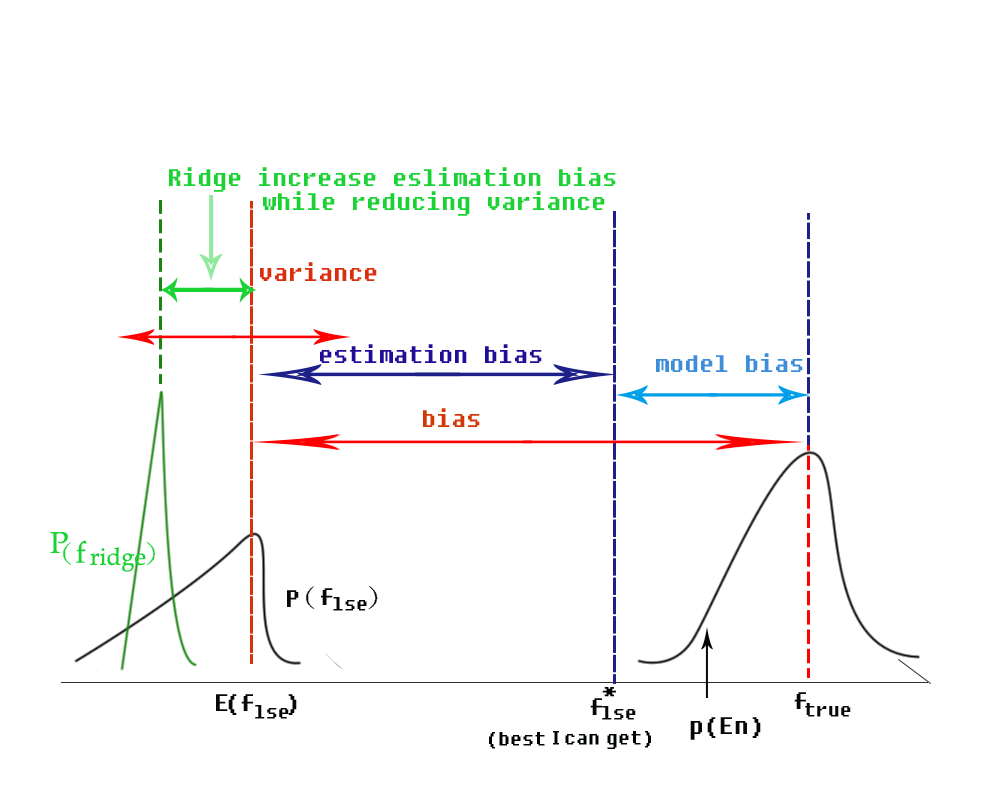
\includegraphics[width=\linewidth]{images/bias-variance2.png}
\end{colfig}

Bias-variance comes directly out of the test error:

 $\bullet$Expected Test Error: $\overline{teErr}$\\
 $= E[(\text{observation} - \text{prediction})^2]  $\\
 $= E_{\mathcal{D}_{tr},\mathcal{D}_{te}}[(y_* - f_{lse})^2]$\\
 $= E_{y_*, \bbeta_{lse}}[(y_* - f_{lse})^2]= $\\
 $E_{y_*, \bbeta_{lse}}[(y_* - f_{true} + f_{true} - f_{lse})^2] $\\
 $=\underbrace{E_{y_*}[(y_* - f_{true})^2]}_{\text{var of measurement}} $\\
 $+ E_{\bbeta_{lse}}[(f_{lse} - f_{true})^2]$ \\
 $=\sigma^2 + E_{\bbeta_{lse}}[(f_{lse} - E_{\bbeta_{lse}}[f_{lse}]$\\
 $ -  f_{true}+E_{\bbeta_{lse}}[f_{lse}] )^2]$ \\
 $=\sigma^2 + \underbrace{E_{\bbeta_{lse}}[(f_{lse} - E_{\bbeta_{lse}}[f_{lse}])^2]}_{\text{pred variance}} $\\
 $+\underbrace{[f_{true}-E_{\bbeta_{lse}}(f_{lse})] ^2}_{\text{pred bias}^2}$\\
 $\bullet reason: E[y_*-f_{true}]=0$
 
 $\bullet$ For least-squares:\\
 $\overline{teErr}=\sigma^2 + \frac{D}{N}\sigma^2 +E_{\bbeta_{lse}}[f_{true}-E_{\bbeta_{lse}}(f_{lse})] ^2]$
 $\Rightarrow D$ increases, variance of estimator increases; N increases, estimation bias decreases.


\begin{tabular}{ l || c | c }
                          & bias & varian \\
  \hline
ridge          & esti bias+    & - \\
simpler model    & +    & - \\
more data               & -    & \\
  \hline
\end{tabular}

% ----------
\section{Classification}
Logistic Function: $\sigma(t) = \frac{exp(t)}{1+exp(t)}$\\
Derivative: $\frac{ \partial\sigma(t) }{ \partial t } = \sigma(t)[ 1 - \sigma(t) ]$

Classification with linear regression: Use $y = 0$ as class $\mathcal{C}_1$
and $y = 1$ as class $\mathcal{C}_2$ and then decide a newly estimated $y$ belongs
to $\mathcal{C}_1$ if $y < 0.5$.

\subsection{Logistic Regression}
$\bullet$ $p(\bf{y}|\bf{X},\bbeta)=\prod_{n=1}^N \sigma(\tilde{\bf{x}}_n^T\bbeta)^{y_n}[1-\sigma(\tilde{\bf{x}}_n^T\bbeta)]^{1-y_n}$

$-\mathcal{L}(\bbeta)=\mathcal{L}_{mle}(\bbeta)=\sum_{n=1}^N[y_n\tilde{\bf{x}}_n^T\bbeta-log[1+exp(\tilde{\bf{x}}_n^T\bbeta)]]$

$\bullet$ $\bf{g}=\frac{ \partial\mathcal{L}_{mle}(\bbeta) }{ \partial \bbeta } =- \tilde{\bf{X}}^T [\sigma(\tilde{\bf{X}} \bbeta) - \bf{y}]$

There's no closed form, we can use gradient descent.

$\bullet$ $\bf{H}(\bbeta) := -\frac{\partial \bf{g}(\bbeta)}{\partial \bbeta^T} 
= \frac{\partial^2 \bf{\mathcal{L}}}{\partial\bbeta\partial\bbeta^T}   
=\sum_{n=1}^N\frac{\partial\sigma(\tilde{\bf{x}}_n^T\bbeta) \tilde{\bf{x}}_n}{\partial \bbeta^T}
=\sum_{n=1}^N\tilde{\bf{x}}_n  \sigma(\tilde{\bf{x}}_n^T\bbeta)[1-\sigma(\tilde{\bf{x}}_n^T\bbeta)]    \tilde{\bf{x}}_n^T
=\tilde{\bf{X}}^T\bf{S}\tilde{\bf{X}} \Rightarrow$ H is \textbf{PSD}.
and with $S_{nn}=\sigma(\tilde{\bf{x}}_n^T\bbeta)[1-\sigma(\tilde{\bf{x}}_n^T\bbeta)]$
and so $\bf{S}=\sigma(\tilde{\bf{X}}\bbeta)[1-\sigma(\tilde{\bf{X}}\bbeta)]^T$.

\subsection{Newton's method}
It uses second order derivatives information and takes steps in the direction that minimizes a quadratic approximation to converge faster.

$\bullet$ $\bf{\mathcal{L}}(\bbeta) \cong \bf{\mathcal{L}}(\bbeta^{(k)})  + g_k^T(\bbeta-\bbeta^{(k)})  + \frac{1}{2}(\bbeta-\bbeta^{(k)})^T\bf{H}_k(\bbeta-\bbeta^{(k)})\Rightarrow  \frac{ \partial\mathcal{L}(\bbeta) }{ \partial \bbeta }=0+g_k+\bf{H}_k(\bbeta-\bbeta^{(k)})=0$
 $\Rightarrow\bbeta^{(k+1)} = \bbeta^{(k)} - \alpha_k \bf{H_k^{-1}} \frac{\partial \mathcal{L}(\bbeta^{(k)})}{\partial \bbeta}$

$\bullet$Newton's method is equivalent to solving many least-squares problems.

Complexity: $\mathcal{O}(I N D^2 + I D^3)$

\subsection{Penalized Logistic Regr}
The cost-function can be unbounded when the data is linearly separable. 

$min_\beta-\sum_{n=1}^Nlogp(y_n|\bf{x}_n^T, \bbeta) + \lambda \sum_{d=1}^D \beta_d^2$
$\Rightarrow $strict convex$(H=\bf{\tilde{X}^TS\tilde{X}}+\lambda\bf{I})$ is positive-definite

\subsection{Iter Recur Leas-Squar}
express Newton's method with $\alpha_k=1$

$\bbeta^{(k+1)} = \bbeta^{(k)}-\alpha_k\bf{H}_k^{-1}\bf{g}_k$
$=\bbeta^{(k)}-(\tilde{\bf{X}}^T\bf{S}_k\bf{\tilde{X}})^{-1}\bf{\tilde{X}}^T(\boldsymbol\sigma_k-\bf{y})$
$=(\tilde{\bf{X}}^T\bf{S}_k\bf{\tilde{X}})^{-1}[(\tilde{\bf{X}}^T\bf{S}_k\bf{\tilde{X}})\bbeta^{(k)}-\bf{\tilde{X}}^T(\boldsymbol\sigma_k-\bf{y})]$
$=(\tilde{\bf{X}}^T\bf{S}_k\bf{\tilde{X}})^{-1}\bf{\tilde{X}}^T\bf{S}_k[\tilde{\bf{X}}\bbeta^{(k)}+\bf{S}_k^{-1}(\bf{y}-\boldsymbol\sigma_k)]$
$=(\tilde{\bf{X}}^T\bf{S}_k\bf{\tilde{X}})^{-1}\bf{\tilde{X}}^T\bf{S}_k\bf{z}_k$
$\Longrightarrow \bbeta^{(k+1)} = argmin_{\bbeta}\sum_{n=1}^NS_{nn}^k(\bf{z}_n^k-\tilde{\bf{x}}_n^k\bbeta)^2$
i.e.$\mathcal{\bf{L}}(\bbeta)= \bf{S}_k(\bf{z}_k-\tilde{\bf{X}}\bbeta)^T(\bf{z}_k-\tilde{\bf{X}}\bbeta)$


\subsection{Generalized linear model}
$\bullet$partition func, natural param, log-partition func
$p(y|\boldsymbol\eta):=\frac{h(y)}{Z(\boldsymbol\eta)}exp[\boldsymbol\eta^T\boldsymbol\Phi(y)-A(\boldsymbol\eta)]$

$\bullet$Logistic Regression: $p(y_n|\eta_n):=\frac{exp(y_n\eta_n)}{1+exp(\eta_n)}=exp[y_n\eta_n-log(1+exp(\eta_n))]$\\

The GLM consists of three elements:
\begin{itemize}
  \item A probability distribution from the exponential family.
  \item A linear predictor $\hat y = \bf{X} \bbeta$ .
  \item A link function g: $E(y) = \mu = g^{-1}(\eta)$.
\end{itemize}

$\bullet$Bernoulli distribution: $p(y|\mu):=\mu^y(1-\mu)^{(1-y)}=exp[y\,log\frac{\mu}{1-\mu}+log(1-\mu)]$

$\frac{\partial A(\eta)}{\partial \eta}=E[\Phi(y)] ,\, \frac{\partial ^2A(\eta)}{\partial \eta^2}=Var(\Phi(y))\Rightarrow$A is convex

$\bullet$Gaussian distribution: $\boldsymbol\Phi(y)=[y, y^2]^T , \, \boldsymbol\eta^T=[\frac{\mu}{\sigma^2}, \frac{-1}{2\sigma^2}] ,\,$
$h(y)=(2\pi)^{-1/2} ,\, Z(\boldsymbol\eta)=(-2\eta_2)^{1/2} ,\, A(\boldsymbol\eta)=\frac{-\eta_1^2}{4\eta_2}$

$\bullet$Multinomial distribution: 

$\bullet$Maximum likelihood estimate:\\
$min\mathcal{L}(\bbeta)=-\sum_{n=1}^Nlog\,p(y_n|\tilde{\bf{x}}_n^T\bbeta)$\\
1. $\mathcal{L}_n(\bbeta)=-logp(y_n|\tilde{\bf{x}}_n^T\bbeta)=-[\eta_n\Phi(y_n)-A(\eta_n)]+cnst$\\
2. $\frac{\partial \mathcal{L}_n}{\partial \bbeta}=\underline{\frac{\partial \eta_n}{\partial \bbeta}\frac{\partial \mathcal{L}_n}{\partial \eta_n}}=\tilde{\bf{x}}_n[g^{-1}(\eta_n)-\Phi(y_n)]$\\
3.vector: $\frac{\partial \bf{\mathcal{L}}}{\partial \bbeta}=\bf{X}^T[g^{-1}(\boldsymbol\eta)-\Phi(\bf{y})]$
4. $\frac{\partial ^2 \bf{\mathcal{L}}(\bbeta)}{\partial \bbeta \partial \bbeta^T}=\bf{X^TSX}$, with $S_{nn}=\frac{\partial ^2 A(\eta_n)}{\partial \eta_n^2}$
always PSD





% ----------
\section{Kernel Ridge Reg}
$\bullet$ $(\bf{P_{NxM}Q_{MxN}}+\bf{I}_N)^{-1}\bf{P}=\bf{P}(\bf{QP+I_M})^{-1}$

$\bullet$ $\bbeta^*=(\bf{X^TX}+\lambda\bf{I}_D)^{-1}\bf{X}^T\bf{y}=\bf{X}^T(\bf{XX}^T+\lambda\bf{I}_N)^{-1}\bf{y}=\bf{X}^T\boldsymbol\alpha^*$\\
complexity: $O(D^2N+D^3)$ $\Rightarrow O(N^2D+N^3)$

$\bullet$\textbf{Representer Theorem}: For any $\bbeta^*$ minimizing
$\min_\beta \sum_{n=1}^N \mathcal{L}(y_n, \bf{x}_n^T \bbeta) + \sum_{d=1}^D \lambda \beta_d^2$
there exists an $\balpha^*$ such that $\bbeta^* = \bf{X}^T \balpha^*$.

$\bullet$Instead of working in the \textbf{column space} of our data, we can work in the \textbf{row space}:
$\bf{\hat{y} = X \bbeta = X X^T \balpha = K \balpha}$


$\bullet\spadesuit$ $\bbeta^*=\bf{X}^T\boldsymbol\alpha^*$ implies for ridge reg that $\bf{x}_*^T\bbeta^*=\sum_{n=1}^N\alpha_n(\bf{x}_*^T\bf{x}_n)$

$\bullet$ $\bbeta^* = \sum_{n=1}^N\alpha_n^*\bf{x}_n \Rightarrow\bbeta^*$ lies in row space of $\bf{X}$

$\bullet$ $\widehat{\bf{y}}=\sum_{d=1}^D\beta_d^*\overline{\bf{x}}_d\Rightarrow\widehat{\bf{y}}$ lies in column space of $\bf{X}$

$\bullet$ $\bbeta^* = arg\,min_{\bbeta}\,\frac{1}{2}(\bf{y}-\bf{X}\bbeta)^T(\bf{y}-\bf{X}\bbeta)+\frac{\lambda}{2}\bbeta^T\bbeta$\\
$\bullet$ $\boldsymbol\alpha^* = arg\,max_{\boldsymbol\alpha} \, -\frac{1}{2}\boldsymbol\alpha^T(\bf{XX}^T+\lambda\bf{I}_N)\boldsymbol\alpha+\boldsymbol\alpha^T\bf{y}$

$\bullet$ Properties of a Kernel:\\
1. $\bf{K}$ should be symmetric: $\bf{K}^T = \bf{K}$\\
  Note: $k(\bf{x}, \bf{x}')=k(\bf{x}', \bf{x})$\\
2. $\bf{K}$ should be PSD: $\forall$ nonzero vector $\bf{a}, \bf{a}^T \bf{K} \bf{a} \geq 0$.

$\bullet$ $t^t\bf{K}t=\sum_i\sum_jK_{ij}t_it_j$


$(\bf{K})_{i,j} = \kappa(\bf{x_i}, \bf{x_j}) = \vec \phi(\bf{x_i})^T \vec \phi(\bf{x_j})$.

$\bullet$ The $\phi$ $\textbf{(basis function)}$ are not that important in the end, because we only use the Kernel as is. 

\begin{tabular}{  | l |}
  \hline
$\kappa(\bf{x_i}, \bf{x_j}) = \bf{x_i}^T \bf{x_j}$ \\
  \hline
$\kappa(\bf{x_i}, \bf{x_j}) = (\bf{x_i}^T \bf{x_j} + c)^d$ \\
  \hline
 $\kappa(\bf{x_i}, \bf{x_j}) = \exp\left(-\frac{||\bf{x_i} - \bf{x_j}||^2}{2\sigma^2}\right)$ \\
  \hline
\end{tabular}



% ----------
\section{SVM}
$\bullet$Cost func(hinge loss):
$g(\bbeta)=$\\
$ \sum_{n=1}^N C[1 - y_n \tilde\phi_n^T \bbeta]_{+} + \frac{1}{2} \sum_{j=1}^M \beta_j^2$

with $[t]_{+} = \max(0, t)$, $C=\frac{1}{\lambda}$ 

$\bullet$Convex, not Differentiable. 

$\bullet$ $\mathcal{G}(\bbeta,\balpha)= \sum_{n=1}^N \alpha_n(1-y_n \tilde\phi_n^T \bbeta) + \frac{1}{2}\sum_{j=1}^M \beta_j^2$

$\bullet$ $\mathcal{G}(\bbeta,\balpha)$ convex in $\bbeta$, concave in $\balpha$
$min_{\bbeta} g(\bbeta)= min_{\bbeta} max_{\balpha} \mathcal{G}(\bbeta,\balpha) = max_{\balpha} min_{\bbeta} \mathcal{G}(\bbeta,\balpha)=max_\alpha g^*(\boldsymbol\alpha)$

$\bullet$ $\max_{\alpha \in [0; C]^N} \balpha^T \bf{1} - \frac{1}{2} \balpha^T \bf{Y \Phi\Phi^T Y} \balpha , \quad \balpha^T \bf{y} = 0, \bf{Y} := diag(\bf{y})$, $\boldsymbol\Phi$ has no first 1 column.

$\bullet$ adv: Differentiable, kernelized, 


% ----------
\section{K-means Clustering}
$\bullet$ $min_{\bf{r}, \boldsymbol\mu} \mathcal{L}(\bf{r}, \boldsymbol\mu) = \sum_{k=1}^K \sum_{n=1}^Nr_{nk}||\bf{x}_n-\boldsymbol\mu_k||_2^2$

$\bullet$ CONVEX with $\boldsymbol\mu$, no notion convex with $\bf{r}$ and $\boldsymbol\mu$

1. For all n, compute $\bf{r}_n$ given $\boldsymbol\mu$\\
$r_{nk}=1$ if k= $arg \, min_{j=1,2,...,K}||\bf{x}_n-\boldsymbol\mu_j||_2^2$

2. For all k, compute $\boldsymbol\mu_k$ given $\bf{r}$
$\mathcal{L}(\boldsymbol\mu_k) = \sum_{n=1}^Nr_{nk}(\bf{x}_n-\boldsymbol\mu_k)^T(\bf{x}_n-\boldsymbol\mu_k)+cnst \Rightarrow$\\
$\frac{\partial \mathcal{L}}{\partial \boldsymbol\mu_k}=-2\sum_{n=1}^Nr_{nk}(\bf{x}_n-\boldsymbol\mu_k)=0$\\
$\Rightarrow \boldsymbol\mu_k = \frac{\sum_{n=1}^N r_{nk}\bf{x}_n}{\sum_{n=1}^N r_{nk}}$

$\bullet$If use $L_1$ distance, called K-median

$\bullet$Complexity: $\mathcal{O}(NKDI)$

$\bullet$Probabilistic model:\\
$-log \, p(\bf{r},\bf{\mu})=\frac{1}{2}\mathcal{L}(\bf{r},\bf{\mu})+cnst$\\
$\Rightarrow p(\bf{r},\boldsymbol\mu)\varpropto exp^{-\frac{1}{2}\sum_k\sum_nr_{nk}||\bf{x}_n-\boldsymbol\mu_k||^2}$
$\prod_n\prod_k[exp^{-\frac{1}{2}||\bf{x}_n-\boldsymbol\mu_k||^2}]^{r_{nk}}\Rightarrow$\\
$p(\bf{r},\boldsymbol\mu)=\prod_n\prod_k[\mathcal{N}(\bf{x}_n|\boldsymbol\mu_k, \mathcal{I})]^{r_{nk}}$



% ----------
\section{Gaussian Mixtu Mode}
GMM is a latent variable model, $\bf{r}_n$ is latent variables

$\bullet$ $p(\bf{X,r} | \bf{\mu},\bf{\Sigma}, \bf{\pi}) = \prod_{n=1}^N [p(\bf{x}_n|\bf{r}_n,\bf{\mu},\bf{\Sigma})p(r_n | \pi)]$ $= \prod_{n=1}^N [\prod_{k=1}^K [\mathcal{N}(\bf{x}_n|\bf{\mu}_k,\bf{\Sigma}_k)]^{r_{nk}}$\\
$ \prod_{k=1}^K [\pi_k]^{r_{nk}}]$

$\bullet$ $p(\bf{x}_n | \theta)$ 
$= \sum_{k=1}^K p(\bf{x}_n, \bf{r}_n=k | \theta) $
$= \sum_{k=1}^K p(\bf{x}_n | \bf{r}_n=k,\theta)p(\bf{r}_n=k | \theta)$
$= \sum_{k=1}^K \pi_k p_{k}(\bf{x}_n |\bf{r}_n=k, \theta) =  \sum_{k=1}^K \pi_k \mathcal{N}(\bf{x}_n | \underbrace{\bf{\mu}_k, \bf{\Sigma}_k}_{\theta})$

$\bullet$ $max_{\theta} \mathcal{L}(\bf{\theta})=$ $max_{\theta} log p(\bf{X} | \bf{\theta})$
$= \sum_{n=1}^N log p(\bf{x}_n | \theta)$
$= \sum_{n=1}^N log \sum_{k=1}^K \bf{\pi}_k \mathcal{N}(\bf{x}_n | \bf{\mu}_k, \bf{\Sigma}_k)$

the negative of it is $\bf{not}$ $\bf{Convex}$ wrt $\theta$, $\bf{not}$ $\bf{Identifiable}$

$\bullet$ To use this for clustering, we first fit this mixture and then compute the posterior $p(z_i = k | \bf{x}_i, \theta)$. This yields \textit{soft} cluster assignments.

% ----------
\section{EM}
$log \sum_{k=1}^K\bf{\pi}_k\mathcal{N}(\bf{x}_n|\bf{\mu}_k,\bf{\Sigma}_k)\geq$ $\sum_{k=1}^Kp_{kn} log\frac{\bf{\pi}_k\mathcal{N}(\bf{x}_n|\bf{\mu}_k,\bf{\Sigma}_k)}{p_{kn}}$

with equality when, 

$p_{kn}=\frac{\bf{\pi}_k\mathcal{N}(\bf{x}_n|\bf{\mu}_k,\bf{\Sigma}_k)}{\sum_{j=1}^K\bf{\pi}_j\mathcal{N}(\bf{x}_n|\bf{\mu}_j,\bf{\Sigma}_j)}$

$\bullet$ 1. E-step: Compute responsibilities $p_{kn}^{(i)}$ 

$p_{kn}^{(i)}= \frac{\bf{\pi}_k^{(i)} \mathcal{N}(\bf{x}_n | \bf{\mu}_k^{(i)}, \bf{\Sigma}_k^{i})}{\sum_{k=1}^K \bf{\pi}_k \mathcal{N}(\bf{x}_n|\bf{\mu}_k^{(i)}, \bf{\Sigma}_k^{(i)}) }$  

$\bullet$ 2. Compute the marginal likelihood (Cost)

$\mathcal{L}(\btheta^{(i)})$ $= \sum_{n=1}^N log \sum_{k=1}^K \bf{\pi}_k^{(i)} \mathcal{N}(\bf{x}_n | \bf{\mu}_k^{(i)}, \bf{\Sigma}_k^{(i)})$

$\bullet$ 3. M-step: Update $\bf{\mu}_k^{(i+1)}$, $\bf{\Sigma}_k^{(i+1)}$, $\bf{\pi}_k^{(i+1)}$

$\bf{\mu}_k^{(i+1)}=$ $\frac{\sum_{n=1}^N p_{kn}^{(i)}\bf{x}_n}{\sum_{n=1}^Np_{kn}^{(i)}}$

$\bf{\Sigma}_k^{(i+1)}=$ $\frac{\sum_{n=1}^N p_{kn}^{(i)}(\bf{x}_n-\bf{\mu}_k^{(i+1)})(\bf{x}_n-\bf{\mu}_k^{(i+1)})^T}{\sum_{n=1}^Np_{kn}^{(i)}}$

$\bf{\pi}_k^{(i+1)}=$ $\frac{1}{N}\sum_{n=1}^Np_{kn}^{(i)}$

EM in general: 
$log p(\bf{x}_n|\btheta)=log\sum_r[\frac{p(\bf{x}_n,\bf{r}|\btheta)}{p(\bf{r}|\btheta^{(i)},\bf{x}_n)}\ast p(\bf{r}|\btheta^{(i)},\bf{x}_n) ]$
$\geq \sum_r[logp(\bf{x}_n, \bf{r}|\btheta)]p(\bf{r}|\btheta^{(i)},\bf{x}_n) + H[p(\bf{r}|\btheta^{(i)},\bf{x}_n)]$

$\Rightarrow\btheta^{(i+1)} = argmax_{\,\theta} $\\
$\sum_{n=1}^N E_{p(\bf{r}_n|\bf{x}_n,\btheta^{(i)})}[log p(\bf{x}_n,\bf{r}_n|\btheta)]$



% ----------
\section{SVD}

$\bullet$ $\bf{X_{DxN}=USV}^T=$ $\sum_{j=1}^Ds_j\bf{u}_j\bf{v}_j^T$. All rank 1.

$\bullet$ $\bf{v}_j^T\bf{v}_j=1,$ $\bf{v}_j^T\bf{v}_i=0,$ $\bf{U}^T\bf{U}=I$ $\bf{V}^T\bf{V}=I$  

$\bigstar$ $\bf{X}\bf{v}_j=s_j\bf{u}_j$

$\bullet$The singular vals of a $D \times N$ matrix $\bf{X}$ are the square roots of the eigenvalues of the $D \times D$ matrix $\bf{X X^T}$ $(D<N)$

$\bullet$The singular vals of a $N \times D$ matrix $\bf{X}$ are the square roots of the eigenvalues of the $D \times D$ matrix $\bf{X^T X}$ $(D<N)$


The same as with PCA, we can do with SVD:
\begin{colfig}
  \centering
  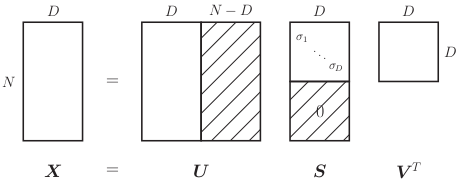
\includegraphics[width=\linewidth]{images/svd.png}
\end{colfig}


\section{PCA}
$\bullet$ $S:=\frac{1}{N}\sum_n(x_n-\overline{x})(x_n-\overline{x})^T$

$\bullet$Find the eigenvectors of the covariance matrix $\bf{X_{DxN} X^T}$ of the data. These form an orthonormal basis $\{ \bf{w}_1, ..., \bf{w}_D\}$ for the data in the directions that have highest variance.
One can then use the first $M < D$ vectors to rebuild the data: $\bf{\hat{x}}_n = \bf{W} \bf{z}_n = \bf{W} \bf{W}^T \bf{x}_n$, with $\bf{W} = \begin{bmatrix} \bf{w}_1 ; ... ; \bf{w}_M \end{bmatrix}$.
This minimizes MSE $\frac{1}{N} \sum_{n=1}^N ||\bf{x}_n - \bf{\hat{x}}_n||^2$.

$\bullet$ $\bf{x}_{n,rot} = \bf{W}^T\bf{x}_n$, $\bf{W}^T\bf{W}=I ,\, \bf{W}\bf{W}^T = I $
$\Rightarrow \bf{x}_n=\bf{W}\bf{x}_{n,rot}$

$\bullet$When use, we use $\tilde{\bf{x}} = \bf{W}^T \bf{x}_i$, which is the lower-dimension approximation to speed up.

$\bullet$Computation Cost:$O(D^3+ND^2+DN^2)??$

\section{PCA, SVD relation}
$\bullet$ $\bf{X}$ is centered(zero mean).\\
$\bullet$ $\bf{XX}^T = \bf{WLW}^{-1} = \bf{US^2U}^T$

$\bullet$ $\hat{\bf{X}}=U(:,1:M)*S(1:M,1:M)*V(:,1:M)^T$



\section{Bayesian methods}
$\bullet$The \textbf{prior} $p(\bf{f}|\bf{X})$ encodes our prior belief about the ``true'' model $\bf{f}$. The \textbf{likelihood} $p(\bf{y}|\bf{f})$ measures the probability of our (possibly noisy) observations given the prior.

$\bullet$Least-squares tries to find model parameters $\bbeta$ which maximize the likelihood. Ridge regression maximizes the \textbf{posterior} $p(\bbeta|\bf{y})$

\subsection{Bayesian networks}
This example can be factorized as follows:
$p(y_1, y_2, z_1, z_2, z_3) = p(y_1 | z_1, z_2) p(y_2 | z_2, z_3) p(z_1) p(z_2) p(z_3)$

\begin{colfig}
  \centering
  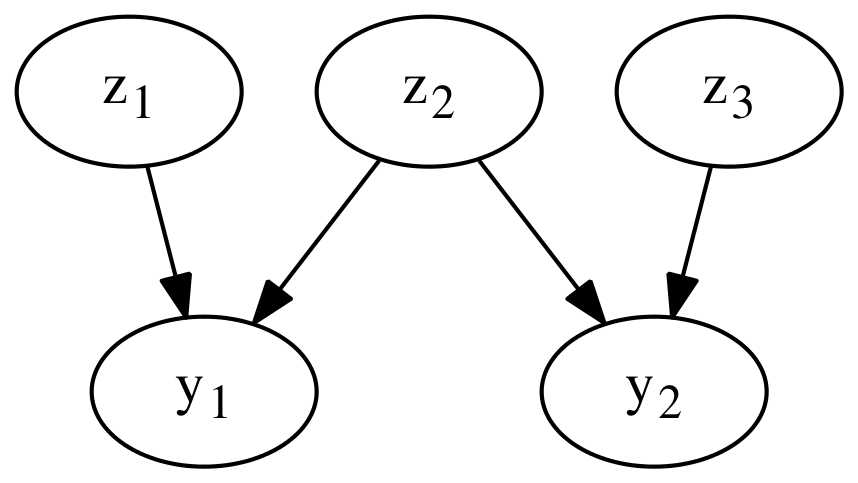
\includegraphics[height=1cm]{images/bayesian-network.png}
\end{colfig}

We can then obtain the distribution over latent factors ($z_i$) by marginalizing over the unknown variables:
$p(z_1, z_2, z_3 | y_1, y_2) = \frac{\text{joint}}{p(y_1, y_2)}$
$\implies p(z_1 | y_1, y_2) = \sum_{z_2, z_3} \frac{\text{joint}}{p(y_1, y_2)}$

$\bullet$Complexity:$\mathcal{O}(2^ME)$ with M is the recursive variables, E is the edges.

$\bullet$Sum-Product Algo: $p(z_1 | y_a, y_b) \propto \sum_{z_2} \sum_{z_3} p(y_a | z_1, z_2) p(y_b | z_2, z_3)$ \\
$p(z_1) p(z_2) p(z_3) =$
$p(z_1)\lbrace\sum_{z_2}p(y_a|z_1, z_2)p(z_2)$\\
$ [\sum_{z_3}p(y_b|z_2, z_3)p(z_3)]   \rbrace$

\subsection{Belief propagation}
$\bullet$z: variables; y: observations

$\bullet$From variables to observations:\\
$m_{i\rightarrow a}(z_i)=p(z_i)\prod_{b\in \mathcal{N}(i)\setminus a}m_{b\rightarrow i}(z_i)$

$\bullet$From observations to variables:\\
$m_{a\rightarrow i}(z_i)=\sum_{j\neq i}$\\
$\lbrace p(y_a|Paret_a) \prod_{j\in \mathcal{N}(a) \setminus i} m_{j\rightarrow a}(z_j)  \rbrace$

$\bullet$1. Initialization: $m_{i\rightarrow a}=p(z_i) \, \forall a$\\
2. Compute marginals by multiplying all the message received at node i.\\
$p(z_i|\bf{y})=p(z_j)\prod_{j\in \mathcal{N}(a)}m_{j\rightarrow a}(z_j)$

$\textbf{The Right One:}$ $p(z_i|\bf{y})=p(z_i)\prod_{a\in \mathcal{N}(i)}m_{a\rightarrow i}(z_i)$


Belief propagation is a message-passing based algorithm used to compute desired marginals (e.g. $p(z_1 | y_1, y_2)$) efficiently. It leverages the factorized expression of the joint. 

% ----------
\section{Neural Networks}
A feed forward Neural Network is organized in $K$ layers, each layer with $M^{(k)}$ hidden units $z_i^{(k)}$. Activations $a_i^{(k)}$ are computed as the linear combination of the previous layer's terms, with weights $\bbeta^{(k)}$ (one $M^{(k-1)} \times 1$ vector of weights for each of the $M^{(k)}$ activations). Activations are then passed through a (possibly nonlinear) function $h$ to compute the hidden unit $z_{in}^{(k)}$.

$\bf{x}_n \xrightarrow{\bbeta_i^{(1)}} a_{in}^{(1)} \xrightarrow{h} z_{in}^{(1)} \xrightarrow{\bbeta^{(2)}} \dots \bf{z}_n^{(K-1)} \xrightarrow{link \,func} \bf{y}_n$

$\bullet$ $a_{in}^{(k)}=(\bbeta_i^{(k)})^T\bf{z}_n^{(k-1)},$\\
$z_{in}^{(k)}=h(a_{in}^{(k)})$

$\bullet$ first layer: $\bf{z}_n^{(0)}=\bf{x}_n$

$\bullet$ $\bf{a}_n^{(k)}=\bf{B}^{(k)}\bf{z}_n^{(k-1)}, \bf{z}_n^{(k)}=h(\bf{a}_n^{(k)})$

\subsection{Backpropagation}
It's an algorithm which computes the gradient of the cost $\mathcal{L}$ w.r.t. the parameters $\bbeta^{(k)}$.

Forward pass: compute $a_i$, $z_i$ and $\bf{y}_n$ from $\bf{x}_n$.

Backward pass: work out derivatives from outputs to the target $\bbeta_i^{(k)}$. Using the chain rule:\\
$\bullet$ $\bdelta_n^{(k-1)} = \frac{\partial \mathcal{L}}{\partial \bf{a}_n^{(k-1)}} = diag[ \bf{h}'(\bf{a}_n^{(k-1)}) ] (\bf{B^{(k)}})^T  \bdelta_n^{(k)}$\\
$\bullet$ $\frac{\partial \mathcal{L}}{\partial \bf{B}^{(1)}} = \bdelta_n^{(1)} \bf{x}_n^T$\\
$\bullet$ $\frac{\partial \mathcal{L}}{\partial \bf{B}^{(k)}} = \bdelta_n^{(k)} (\bf{z}_n^{(k)})^T$

\subsection{Regularization}
NN are not \textit{identifiable} (existence of many local optima), therefore the maximum likelihood estimator is not \textit{consistent}.

NN are universal density estimators, and thus prone to severe overfitting. Techniques used to reduce overfitting include early stopping (stop optimizing when test error starts increasing) and ``weight decay'' (i.e. $L_2$ regularization).





% ----------
\section{General}

\subsection{Cost functions}
%\begin{colfig}
%\centering
%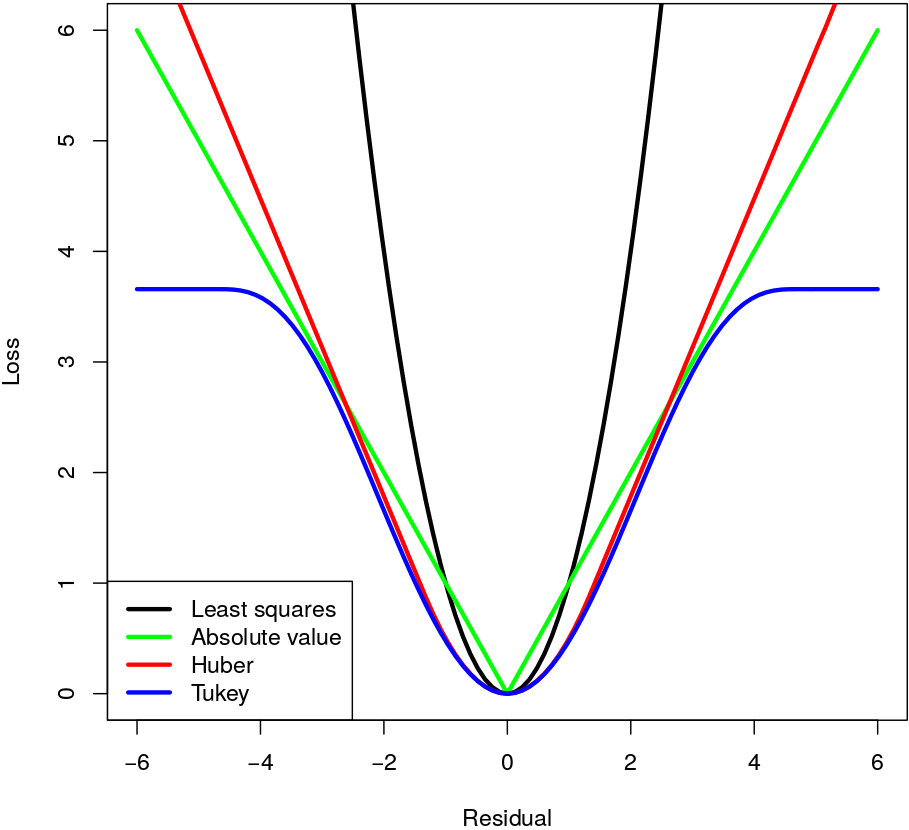
\includegraphics[width=\linewidth]{images/error-functions.png}
%\end{colfig}


$\bullet$MSE(and matrix formulation): $\frac{1}{2N} \sum_{n=1}^{N}\left[y_n-f(\bf{x}_i) \right]^2$
$=\frac{1}{2N} (\bf{y - X \bbeta})^T (\bf{y - X \bbeta})$

$\bullet$Mean absolute error (MAE): $\frac{1}{2N} \sum_{n=1}^{N}\left | y_n-f(\bf{x}_i) \right |$

$\bullet$Huber loss(convex, differentiable, robust to outliers): 
$\mathcal{L}_\delta (a) = \begin{cases}
\frac{1}{2}{a^2}                   & \text{for } |a| \le \delta, \\
\delta (|a| - \frac{1}{2}\delta ), & \text{otherwise.}
\end{cases}$

$\bullet$Turkey's loss(non-convex, non-differentiable, robust to outliers)

$\bullet$RMSE: $\sqrt{2 * \text{MSE}}$

$\bullet$Epsilon insensitive (``hinge loss''):
$\mathcal{L}_{\epsilon}(y, \hat{y}) = \begin{cases}
0                   & \text{if } |y - \hat y| \le \epsilon, \\
|y - \hat y| - \epsilon, & \text{otherwise.}
\end{cases}$

\subsection{Classif Cost functions}
RMSE: $\sqrt{\frac{1}{N} \sum_{n=1}^{N}\left[y_n- \hat{p_n} \right]^2}$

0-1 Loss: $ \frac{1}{N} \sum_{n=1}^{N} \delta(y_n, \hat{y_n})$

Log-Loss: $- \frac{1}{N}  \sum_{n=1}^{N} y_n \log(\hat{p_n}) + (1-y_n) \log(1-\hat{p_n})$

\subsection{Distributions}
$\bullet$Multivariate gaussian distribution:\\
 $\mathcal{N}(\bf{X} | \bf{\mu} , \bf{\Sigma})$ 
$= p(\bf{X} = \bf{x}) =$\\
$(2 \pi)^{-d/2} |\bf{\Sigma|}^{-1/2}$\\
$ \exp{[- \frac{1}{2} (\bf{x} - \bf{\mu})^T \bf{\Sigma}^{-1} (\bf{x} - \bf{\mu})]}$

$\bullet$Gaussian distribution: \\
$\mathcal{N}(X| \mu, \sigma^2)$ 
$= p(X = x) = \frac{1}{\sqrt{2 \pi \sigma^2}} \exp{(- \frac{1}{2} ( \frac{x - \mu}{\sigma} )^2)}$

$\bullet$Poisson distribution: $\mathcal{P}(X| \lambda)$ \\
$\implies p(X = k) = \frac{\lambda ^ k}{k!} \exp{(- \lambda)}$

$\bullet$Laplace distribution: $p(y_n|\tilde{\bf{x}}_n,\boldsymbol\beta)=\frac{1}{2b}e^{\frac{1}{b}|y_n-\tilde{\bf{x}}_n^T\boldsymbol\beta|}$

\subsection{Properties}
$\bullet$ If $\bf{V}$ symmetric positive definite, then for all $\bf{P} \neq 0$, $\bf{P^T V P}$ is positive semi-definite (and even positive definite if $\bf{P}$ is not singular).

$\bullet$\textbf{Jensen's inequality} applied to $\log$: $\log( \mathbb{E}[X] ) \geq \mathbb{E}[\log(X)]$ \\
$\implies \log ( \sum_x x \cdot p(x) ) \geq \sum_x p(x) \log(x)$


$\bullet$Useful derivative: $\frac{\partial \bf{x^T B x}}{\partial \bf{x}} = (\bf{B + B^T}) \bf{x}$

$\bullet$ \textbf{Marginal and Conditional Gaussians:}

$p(\bf{x}) = \mathcal{N}(\bf{x} | \boldsymbol\mu, \boldsymbol\Lambda^-1) $\\
$p(\bf{y}|\bf{x}) = \mathcal{N}(\bf{y} | \bf{Ax + b, L}^-1)$ \\
$\Downarrow$ \\
$p(\bf{y}) = \mathcal{N}(\bf{y} | \bf{A} \boldsymbol\mu + \bf{b}, \bf{L}^-1 + \bf{A} \boldsymbol\Lambda^-1 \bf{A}^T)$	\\
$p(\bf{x}|\bf{y}) = \mathcal{N}(\bf{x} |\boldsymbol\Sigma \{ \bf{A^T L(y - b) + \Lambda \mu} \}, \boldsymbol\Sigma)$ \\
\text{where } $\boldsymbol\Sigma = (\boldsymbol\Lambda + \bf{A^T L A})^{-1}$

$\bullet$ \textbf{derivative for expo like PDF}: $\frac{\partial f(x)}{\partial x}=\frac{\partial e^{lnf(x)}}{\partial x}=f(x)\frac{\partial lnf(x)}{\partial x}$


% ----------
\section{Concepts}

\subsection{Convexity}

Sum of two convex functions is convex. Composition of a convex function with a convex, nondecreasing function is convex. Linear, exponential and $\log(\sum \exp)$ functions are convex.



\subsection{Identifiability}
We say that a statistical model $\mathcal{P} = \{P_\theta: \theta \in \Theta\}$ is identifiable if the mapping $\theta \mapsto P_\theta$ is one-to-one:
$P_{\theta_1}=P_{\theta_2} \quad\Rightarrow\quad \theta_1=\theta_2 \quad\ \text{for all } \theta_1,\theta_2\in\Theta.$

A non-identifiable model will typically have many local optima yielding the same cost, e.g. $\mathcal{L}(W, Z) = \mathcal{L}(aW, \frac{1}{a} Z)$

$\bullet$ check permutation of labels.

\subsection{Curse of dimensionality}
With the dimensionality increase, every data point becomes arbitrarily far
from every other data point and therefore the choice of nearest neighbor becomes random.
In high dimension, data only covers a tiny fraction of the input space, making generalization extremely difficult.

$\bullet$ expected edge length = $e_D(r)=r^{1/D}$; $e_{10}(0.1)$=0.80, to capture 10\% of data, must cover 80\% of input.

$\bullet$The median distance from the origin to the closest data point is: $(1-\frac{1}{2}^{1/N})^{1/D}$. choice of KNN becomes random.


\section{Maximum Likelihood}
$\bullet$ $\bbeta_{lse} = arg \, min_\beta \frac{1}{2}(\bf{y}-\tilde{\bPhi}\bbeta)^T(\bf{y}-\tilde{\bPhi}\bbeta)$\\
$=arg \, max_\beta[log\mathcal{N}(\bf{y}|\tilde{\bPhi}\bbeta,\bf{I})]$

$\bullet$ $\bbeta_{ridge} = arg \, min_\beta \frac{1}{2}(\bf{y}-\tilde{\bPhi}\bbeta)^T(\bf{y}-\tilde{\bPhi}\bbeta)+\frac{1}{2}\lambda\bbeta^T\bbeta=$\\
$arg \, max_\beta[log\mathcal{N}(\bf{y}|\tilde{\bPhi}\bbeta,\bf{I})\mathcal{N}(\bbeta|\bf{0}, \frac{1}{\lambda}\bf{I})]$

$\bullet$multinomial: $p(\bf{x}_n|\boldsymbol\mu)=\prod_{k=1}^K\mu_k^{x_k}=exp[\sum_{k=1}^Kx_kln\,\mu_k]=$
$exp[\sum_{k=1}^{K-1}x_kln(\frac{\mu_k}{1-\sum_{j=1}^{K-1}}) + ln(1-\sum_{k=1}^{K-1}\mu_k)]$, with $\sum_{k=1}^{K}\mu_k=1$, $E[\bf{x}]=\boldsymbol\mu$,
$\sum_{k=1}^{K}x_k=1, x_k=1$.

\section{Matrix Factorization}
$\bullet$ $\bf{X}_{D*N}=\bf{W}_{D*M}\bf{Z}_{N*M}^T$, with M is the num of factors.

$\bullet$ $\bf{\mathcal{L}}(\bf{W},\bf{Z})=\frac{1}{2}\sum_{n=1}^N\sum_{d=1}^D(x_{dn}-\bf{w}_d^T\bf{z}_n)^2$
$+\frac{\lambda_w}{2}\sum_{d=1}^D\bf{w}_d^T\bf{w}_d$
$+\frac{\lambda_z}{2}\sum_{n=1}^N\bf{z}_n^T\bf{z}_n$

$\bullet$ $\bf{\mathcal{L}}(\bf{Z}|\bf{W})=\frac{1}{2}\sum_{n=1}^N[(\bf{x}_n-\bf{W}\bf{z}_n)^T(\bf{x}_n-\bf{W}\bf{z}_n)]+\lambda_z\bf{z}_n^T\bf{z}_n$

$\bullet$ $\bf{z}_n^*=(\bf{W}^T\bf{W}+\lambda_z\bf{I})^{-1}\bf{W}^T\bf{x}_n$
$\bf{w}_d^*=(\bf{X}^T\bf{Z}+\lambda_w\bf{I}_M)^{-1}\bf{Z}^T\bf{x}_d$
$\bf{Z}^T=(\bf{W}^T\bf{W}+\lambda_z\bf{I}_M)^{-1}\bf{W}^T\bf{X}$
 $\Rightarrow\mathcal{O}((M^2D+M^3)N)$
$\bf{W}^T=(\bf{Z}^T\bf{Z}+\lambda_w\bf{I}_M)^{-1}\bf{X}^T\bf{X}^T$
 $\Rightarrow\mathcal{O}((M^2N+M^3)D)$
 
$\bullet$ $\prod_{n=1}^N\prod_{d\in O_n}N(x_{dn}|\bf{w}_d^T\bf{z}_n,1)\prod_nN(\bf{z}_n|\bf{0},\frac{1}{\lambda_z}\bf{I})\prod_dN(\bf{w}_d|\bf{0},\frac{1}{\lambda_w}\bf{I})$

\section{Decision Tree}
$\bullet$ $L=(x_i,y_i),\, s.t. \, x_{ik}\succ \tau, \, R... $\\
$\bullet$ $p_L=\frac{\sharp y_i=1}{N_L},\, p_R...$\\
$\bullet$ $I_{split} = N_L I(p_L)+N_RI(p_R)$\\
$\bullet$ Cross-entropy = I(p)\\
$\bullet$ gini impurity = 2p(1-p)\\
$\bullet$ regr impuri=$\frac{1}{N_{L,R}}\sum_n(y_n-\overline{y})^2$ 












\end{multicols*}
\end{document}
